%%%%%%%%%%%%%%%%%%%%%%%%%%%%%%%%%%%%%%%%%%%%%%%%%%%%%%%%%%%%%%%%%%%%%%%%%%%%%%%%
%2345678901234567890123456789012345678901234567890123456789012345678901234567890
%        1         2         3         4         5         6         7         8

\documentclass[letterpaper, 10 pt, conference]{ieeeconf}  % Comment this line out if you need a4paper

%\documentclass[a4paper, 10pt, conference]{ieeeconf}      % Use this line for a4 paper

\IEEEoverridecommandlockouts                              % This command is only needed if
                                                          % you want to use the \thanks command

\overrideIEEEmargins                                      % Needed to meet printer requirements.

%In case you encounter the following error:
%Error 1010 The PDF file may be corrupt (unable to open PDF file) OR
%Error 1000 An error occurred while parsing a contents stream. Unable to analyze the PDF file.
%This is a known problem with pdfLaTeX conversion filter. The file cannot be opened with acrobat reader
%Please use one of the alternatives below to circumvent this error by uncommenting one or the other
%\pdfobjcompresslevel=0
%\pdfminorversion=4

% See the \addtolength command later in the file to balance the column lengths
% on the last page of the document

% The following packages can be found on http:\\www.ctan.org
\usepackage{graphicx} % for pdf, bitmapped graphics files
%\usepackage{epsfig} % for postscript graphics files
%\usepackage{mathptmx} % assumes new font selection scheme installed
%\usepackage{times} % assumes new font selection scheme installed
\usepackage{amsmath} % assumes amsmath package installed
\usepackage{amssymb}  % assumes amsmath package installed
%\usepackage{dsfont}
\usepackage{algorithm}
\usepackage{algorithmic}
\usepackage{commath}

\usepackage{xcolor}
\newcommand{\todo}[1]{{\color{blue}[TODO: #1]}}
\newcommand{\response}[1]{{\color{green}[RESPONSE: #1]}}

\DeclareMathOperator*{\argmax}{arg\,max}
\DeclareMathOperator*{\argmin}{arg\,min}

\title{\LARGE \bf
Optimal Coverage with Genetic Path Planning
}


\author{Jacob M. Olson$^{1}$, Craig C. Bidstrup, Brady K Anderson,Which Professors?$^{2}$% <-this % stops a space
\thanks{This research was supported through the Center for Unmanned Aircraft Systems (C-UAS), a National Science Foundation-sponsored industry/university
cooperative research center (I/UCRC) under NSF Award No. IIP-1650547
along with significant contributions from C-UAS industry members.}% <-this % stops a space
\thanks{$^{1}$The corresponding author can be contacted at
        {\tt\small  at byu.edu}.}%
\thanks{$^{2}$All authors are with the Department of Mechanical Engineering or Electrical and Computer Engineering,
        Brigham Young University, Provo, UT, 84602, USA.}%
%\thanks{$^{3}$C. Peterson is with the Faculty of Electrical and Computer Engineering,
%		Brigham Young University, Provo, UT, 84602, USA.
%        {\tt\small cammy.peterson at byu.edu}}%
%\thanks{$^{4}$R. W. Beard is with the Faculty of Electrical and Computer Engineering,
%		Brigham Young University, Provo, UT, 84602, USA.
%        {\tt\small beard at byu.edu}}%
}



\begin{document}



\maketitle
\thispagestyle{empty}
\pagestyle{empty}


%%%%%%%%%%%%%%%%%%%%%%%%%%%%%%%%%%%%%%%%%%%%%%%%%%%%%%%%%%%%%%%%%%%%%%%%%%%%%%%%
\begin{abstract}

When generating 3D maps with unmanned arial vehicles (UAVs), it is important to the mapping algorithms to have good coverage of the environment and have multiple loop closures throghout the flight path. Because multirotor UAVs are limited in flight time, the flight paths must not be too long. Coming up with a good flight path of a new environment to be mapped can be difficult to do well and becasue of how free-form a flight path can be, it is also tricky to generate optimal paths to get good coverage with minimal flight time.
To solve this problem, we propose using a genetic algorithm designed to maximize total area coverage while minimizing flight time. Because of the more randomized searching that genetic algorithms have, it is more capable of solving complex free-form problems like path planning.

\end{abstract}


%%%%%%%%%%%%%%%%%%%%%%%%%%%%%%%%%%%%%%%%%%%%%%%%%%%%%%%%%%%%%%%%%%%%%%%%%%%%%%%%
\section{INTRODUCTION}

%Talk about lit review and what we will be contributing to the space

%add multi agent to this
Autonomously generating an internal 3D map of a building requires intelligent control of the mapping vehicle. This ranges from manually planning a flight path with simple obstacle avoidance to full stack exploration and path planning algorithms.

Generating a flight path is a nontrivial task especially when multiple objectives are considered. For example, the algorithm may want to maximize observed coverage of the space while minimizing flight time. This becomes tedious with each new space and more difficult as the complexity of the space increases with more rooms and inter-connecting hallways. When planning paths to achieve good coverage of the area rather than obstacle avoidance or traversability, it becomes much more complex. To plan effective flight paths in more complex flight spaces, using algorithms to plan the paths becomes a necessity.

The complexity of the design space renders many simple optimization routines improper for this problem. We chose to use a genetic algorithm because they better handle the design complexity of this type of problem. Further, by the structure of the problem, derivatives were not available for each design variable. Thus, a derivative-free approach was required.

We first discretized and simplified the problem as much as possible to shrink the design space before applying a genetic algorithm. We found our genetic algorithm was able to effectively plan paths in an arbitrary environment and satisfy the constraints of the problem.

The remainder of the paper is organized as follows: Section \ref{setup} describes the method for simplifying the design space to create a reasonable problem for the genetic algorithm to solve. Section \ref{approach} describes the approach and architecture used to generate optimal paths for a single UAV.
%, then the method is extended to multi-agent path planning.
Results showing and evaluating the generated paths are presented in Section \ref{results}. Finally, conclusions are presented in Section \ref{conclusions}.

%%%%%%%%%%%%%%%%%%%%%%%%%%%%%%%%%%%%%%%%%%%%%%%%%%%%%%%%%%%%%%%%%%%%%%%%%%%%%%%%
\section{OPTIMIZATION SETUP}\label{setup}


Modeling a problem for optimization requires a balance between fidelity and tractability. Model accuracy is especially important because any inaccuracies in the model can lead to solutions that are not truly optimal in the physical system. However, if the design space is too large, or ill formed, optimization algorithms can fail to converge especially when derivatives are not available or there are multiple local optima.

\subsection{Problem Statement}

The goal of our optimization is to generate a path through a simple floor plan with the intent of building a 3D map using a UAV and an RGB-D (color and depth) camera. We start with a simple 2D floor plan of the area of interest and a known scale of the map. With as little human interaction as possible, the objective is to generate a flight path for the UAV to map the building, maximizing coverage while minimizing flight time so that the path is feasible with real hardware.

\subsection{Discretization}

The open-ended nature of path planning makes it a difficult problem for optimization. To simplify the design space we discretize it as much as possible.

\subsubsection{Map Generation}

The first step to discretizing the design space is to simplify the 2D floor plan. The only part of discretization that must be done manually is differentiating between areas to be explored (explorable) and inaccessible or uninteresting areas (occluded) on the 2D map. Fig. \ref{fig:map_gen} illustrates how this differentiation works. The white space represents the explorable area and black space is the occluded area such as walls or inaccessible rooms.

\begin{figure}
\centering
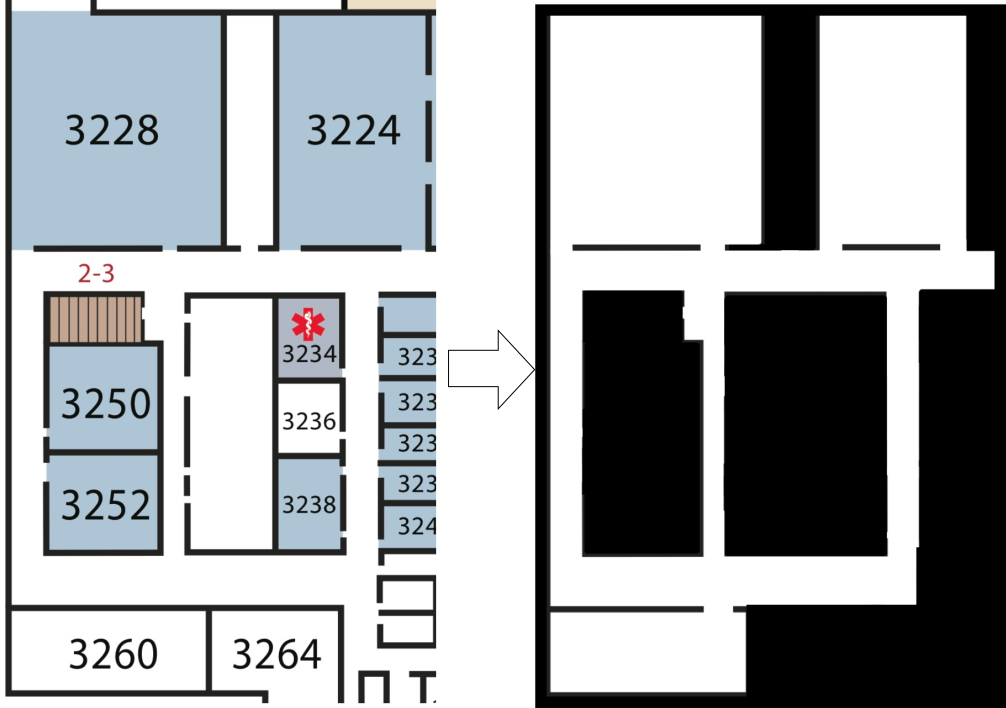
\includegraphics[width=0.8\linewidth]{figures/map_bw.png}
\caption{The initial 2D floor map of the area of interest and the segmented floor map reflecting explorable and occluded spaces}
\label{fig:map_gen}
\end{figure}

Once this map is segmented, the user passes it into the map generator along with the scale from pixels to meters and the width of the narrowest hallway.

The map generator then takes the obstacle map and scales it down so that each pixel represents the minimum resolution desired in the optimization. This value could be adjusted to balance run time and fidelity. Once the map is properly scaled it is passed to the waypoint generator.

\subsubsection{Waypoints}

To further discretize and simplify the design space of the optimization, we place waypoints on the map and constrain the flight path to only fly through these waypoints. First, a grid is overlaid onto the map with a resolution of one half the width of the narrowest flyable hallway. This ensures that there are waypoints in every hallway and room so that the space is fully traversable. Next, all waypoints overlapping occluded space are removed.

After removing occluded waypoints, the remaining waypoints are further pruned and adjusted to better cover the space. To remove waypoints that would cause the UAV to collide with obstacles, we generate a safety buffer around all occluded space at least half the width of the UAV. Any waypoint that falls within this safety buffer is nudged away from the wall. Then waypoints are pruned one last time to remove redundancy. The distance between adjacent waypoints is checked and any that are closer than the initial grid resolution are replaced with a single waypoint at the centroid of the cluster. This prevents over crowding of waypoints in hallways and corners to make it simpler to generate flight paths through narrow hallways and near walls in rooms. Fig. \ref{fig:waypoints} shows an example of this waypoint pruning process. Point A is an example of two waypoints being replaced by a single one and Point B is an example of three waypoints being replaced by a single one.

\begin{figure}
\centering
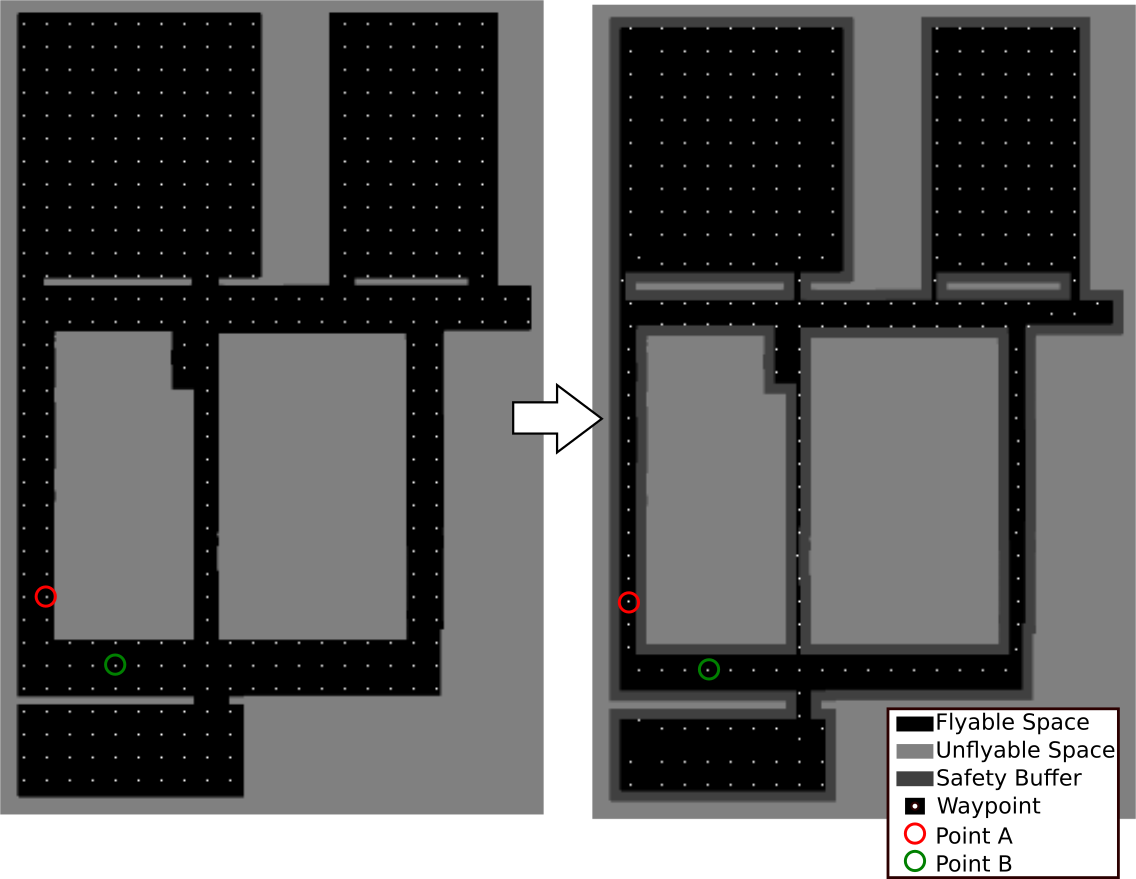
\includegraphics[width=0.8\linewidth]{figures/waypoint2.png}
\caption{The initial waypoint grid with only occluded waypoints removed on the left, The modified waypoint grid with safety buffer and anti-crowding on the right.}
\label{fig:waypoints}
\end{figure}

\subsection{Objective Functions}

We split the optimization into two competing objectives. First, to maximize coverage of the given map, and second, to minimize flight time.

\subsubsection{Maximize Coverage}

The first objective is to maximize coverage of the environment.  To simplify the problem, we assumed that the UAV would only fly forward. Using the minimum and maximum viewable depths and horizontal field of view  we create the camera viewable area. At each waypoint, with its orientation, we set the currently viewable area as explored. After doing that for every waypoint, we calcualte the percent of the explorable space in the map that is seen in that path and use that value as the first objective function. See Fig. \ref{fig:coverage} for an example result of this step.

\begin{figure}
\centering
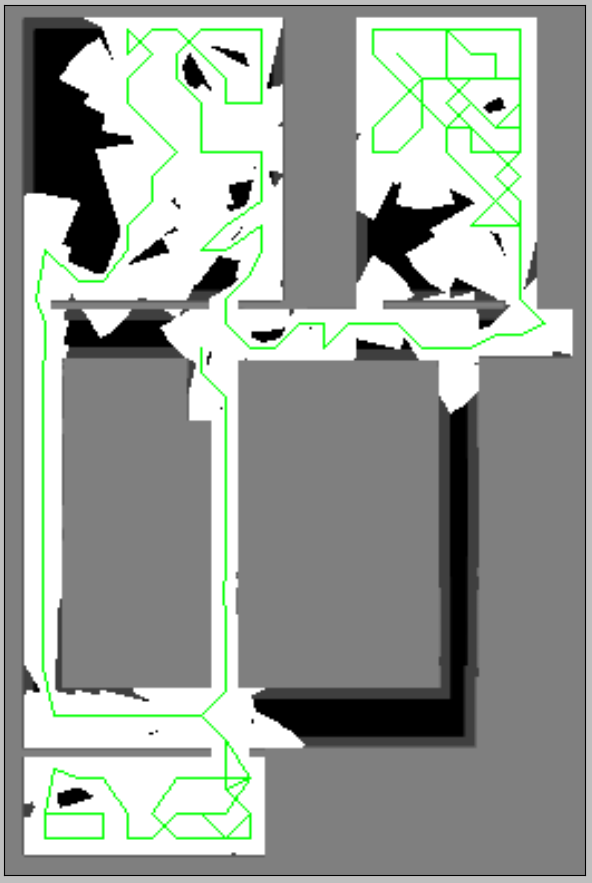
\includegraphics[width=0.8\linewidth]{figures/coverage_map2.png}
\caption{An example path and its corresponding coverage. The green line is the path flown, light grey represents obstacles, white represents explored area, and black and dark grey represent unexplored area}
\label{fig:coverage}
\end{figure}


\subsubsection{Minimize Flight Time}

The second objective function minimizes flight time. To achieve this, we assume a constant velocity flight and compute the total distance flown in each path. This way, paths with fewer waypoints are considered more fit according to the objective function.

\subsection{Traversable Graph}

which defines the possible waypoints are reachable from each waypoint

This graph defines to which waypoints the UAV can travel from the current waypoint position

To save computation when generating or modifying paths, we pre-compute the traversability graph. The UAV is allowed to move to any waypoint defined in the traversability graph for its current position. For any given waypoint we want to constrain movement only to adjacent waypoints that are not obscured by obstacles. To achieve this, we split up the space around each waypoint into octants. Then, we find the nearest waypoint in each octant and add an edge between it and the current waypoint. To prevent flying into obstacles, we prune the graph to remove any traversing that collides with obstacles with a simple line intersection algorithm.

Using this traversability graph, we generate feasible paths for the UAV. Passing in the desired path length and the starting location, it randomly chooses the next waypoint from the traversability graph. The probability of choosing the next waypoint favors forward motion, with probability falling off as turning angle increases to prevent too much meandering. To reduce backtracking, we also encoded a short term memory so that the UAV will not return to a recent waypoint unless there is no other choice.

%%%%%%%%%%%%%%%%%%%%%%%%%%%%%%%%%%%%%%%%%%%%%%%%%%%%%%%%%%%%%%%%%%%%%%%%%%%%%%%%
\section{APPROACH}\label{approach}
\subsection{Single Agent Architecture}

\subsubsection{Chromosome}

The chromosome defining each member organism in a generation has a minimum, initial, and maximum number of genes. Each gene represents one waypoint in a path and its value encodes a location in the grid of possible waypoints, as seen in Fig. \ref{fig:waypoints}. The first generation of parents is spawned by generating a random path within the 2D map. The first step to create this path is to seed the same initial waypoint to each organism in the generation's population, representing the idea that the doorway to enter the building is always in the same place. Thus, whatever random path may be considered most optimal, it must always start at the entrance. Next, each consecutive gene, or waypoint, is generated by using the traversable graph to find a valid next waypoint. All organisms in the first generation start with the same initial number of waypoints, however, the chromosome length is allowed to vary in crossover and mutation between the minimum and maximum number of genes. Once the chromosome is defined, both the coverage and flight time objective values are computed for that organism.

\subsubsection{Crossover}

Given a set of two parents, crossover creates two children. Crossover occurs with a defined probability. If crossover does not occur, the children are clones of the parents. Otherwise, a search is done along the length of both chromosomes to determine where, if at all, both paths cross through the same waypoint. Next, one of the common waypoints is randomly chosen, and the tails of the chromosomes are swapped. See Fig. \ref{fig:crossover} for an example. If at any point a chromosome becomes longer than the maximum allowable length, it is truncated to the maximum length. In contrast, if the chromosome becomes shorter than the minimum allowable length, the chromosome is lengthened with a random feasible path up to the minimum chromosome length.

\begin{figure}
\centering
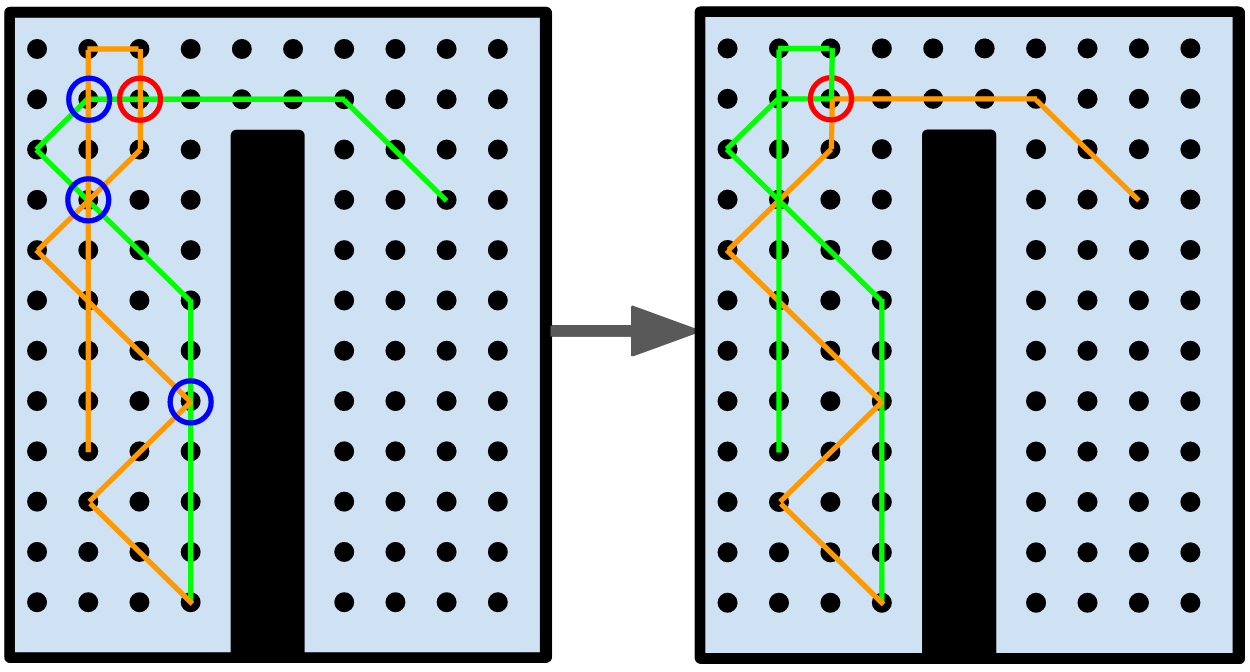
\includegraphics[width=0.8\linewidth]{figures/crossover.png}
\caption{An example of the crossover mechanism. First, common waypoints are found (marked in blue and red). Next, one of the common waypoints is chosen at random (red). Finally, the tails of the two paths are swapped, as shown on the right.}
\label{fig:crossover}
\end{figure}

\subsubsection{Mutation}

After a new chromosome is generated, either by cloning or crossover, it is subjected to two different types of mutation, each with a defined probability of occurring. The first type of mutation randomly selects both a random gene in the chromosome and a random length between the current and maximum chromosome length. Using the traversable graph, a new path is randomly generated from that gene onward, up to the randomly chosen length. See Fig. \ref{fig:mutation} for an example of this style of mutation.

\begin{figure}
\centering
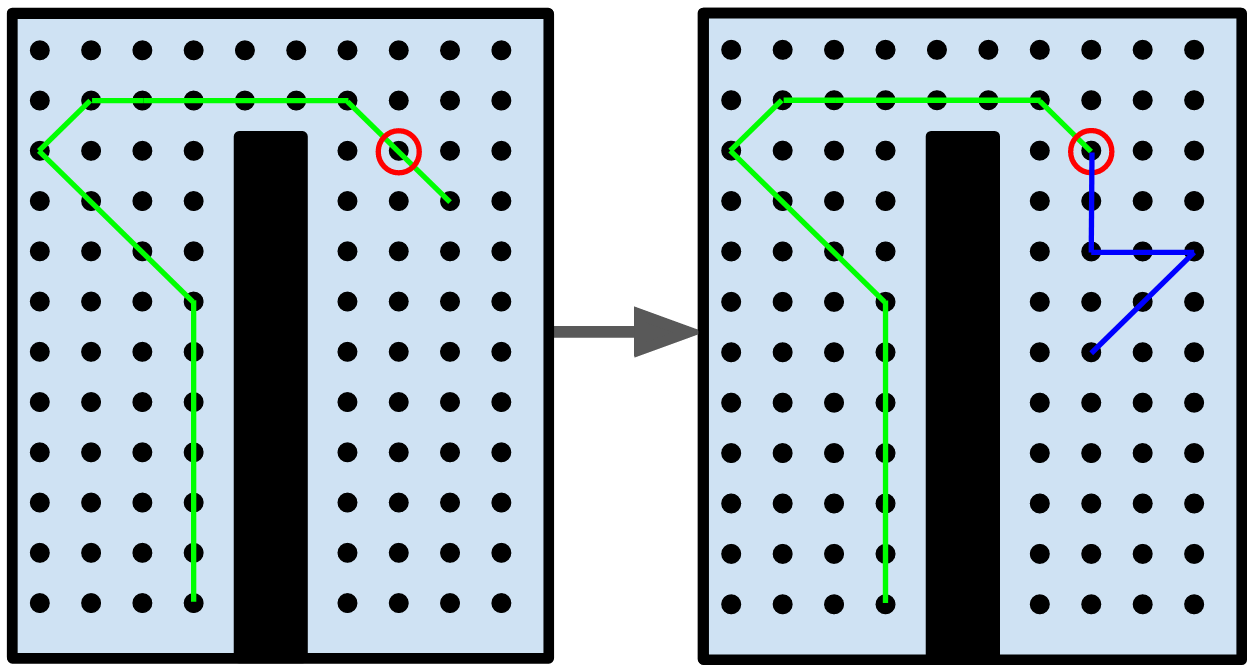
\includegraphics[width=0.8\linewidth]{figures/mutation.png}
\caption{An example of the Mutation B mechanism. A random waypoint in the path is chosen (marked in red) and the tail is replaced with a random path of a random length.}
\label{fig:mutation}
\end{figure}

The second mutation is intended to straighten and shorten the paths. A random segment (random in position, static in length) of the chromosome is selected. The hamming distance from the first waypoint in the segment to all other waypoints in the segment, starting with the last point, is computed. If a point is found to be within two waypoints of the first point in the segment, all waypoints in the segment between those two are replaced with a shortcut, as illustrated in Fig. \ref{fig:muterpolation}. However, this is only completed according to a defined sub-probability of mutation, which is typically much higher than the overall mutation probability. The segment is left as is if no points are within a hamming distance of two. This type of mutation is applied to the chromosome a specified number of times with the intent of finding multiple useful shortcuts in the path.

\begin{figure}
\centering
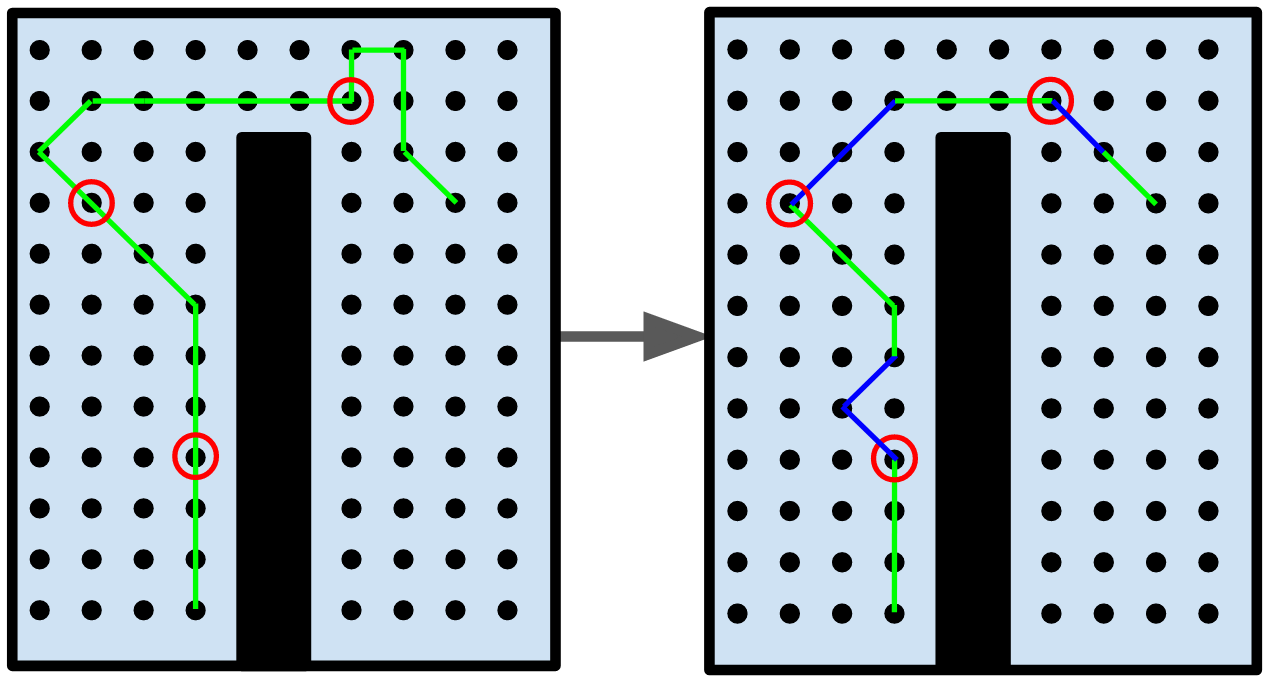
\includegraphics[width=0.8\linewidth]{figures/muterpolation.png}
\caption{An example of the Mutation B mechanism. Multiple random points are chosen (marked in red). From each point, the path is searched up to a certain length to find places where shortcuts or alternate paths can be taken (shown as blue segments).}
\label{fig:muterpolation}
\end{figure}

\subsubsection{Constraints}

Most of the constraints of the system are modeled into the discretization, traversability graph, and upper and lower bounds of the chromosome length. however constraining the minimum coverage could not be applied directly to the model.

The coverage constraint was applied by adding to the cost to make it worse than the worst feasible design. Since we are using two objectives we implemented this constraint by adding a large cost to the flight time objective to guarantee that all organisms violating the constraint will be dominated by other designs (according to the maximin fitness).

Rather than start with a high constraint that would eliminate many of the original designs, we initialized the constraint with a low value. Over several generations we increase the constraint slowly to push the designs into the desired region of objective space. This also inadvertently increases the average flight time, but as the system continues to evolve, more efficient flight paths are found even with the new, strict coverage constraint.

As described in \cite{Parkinson2019}, constraints are applied to the fitness value. Because we have two objectives, and our non-modeled constraint directly relates to only one of the objectives, we implement this constraint on the objective value prior to computing the fitness value for the organism.

\subsubsection{Minimax and Elitism}

After all of a generation's children have been created, The fitness of the parents and children is computed by using the minimax fitness function. In brief, the minimax scheme encourages a spread of designs across the Pareto front between competing objective values, with a target of minimizing the objectives. It does this by calculating the distance between each of the objective values of all the organisms, and finds the minimum difference of both objectives to each other. It then computes the maximum of all of those minima as the fitness value. Following the notation in \cite{Parkinson2019}, if $f_k^i$ is the computed $k^{\mathrm{th}}$ objective value for organism $i$, the minimax fitness for organism $i$ is computed by,
\begin{equation}%\nonumber
    fitness = \max_{i \neq j}\left(\min_{k}\left(f_k^i - f_k^j\right)\right).
\end{equation}

Once all parents and children have fitness values computed with respect to each other, the best $N$, comprising of the most negative fitness values, is selected as the next generation, where $N$ is the size of a generation.

\subsubsection{Low-Variance Sampling}

We use a Roulette-style sampling method to pick parents in a way that gives organisms with better designs (determined by the maximin fitness) a higher probability of being selected as a parent for the crossover process. We employ a low-variance sampling technique as described in \cite{Thrun2006}. This method normalizes the population's fitnesses and treats them as a set of probabilities. A naive approach randomly samples $N$ times from the pool of parents according to their respective probabilities. In order to reduce the possibility of a parent being sampled disproportionately to its probability, we draw as single uniform random number $r$ between 0 and $\tfrac{1}{N}$. The probabilities are then stacked up and compared to $r$. Whichever organism corresponds to the bin that $r$ falls into gets sampled and $\tfrac{1}{N}$ is added to $r$ and again compared to the stack of probabilities. This process is repeated $N$ times.


%\subsection{Multi-Agent Architecture}
%\subsubsection{Chromosome}
%\subsubsection{Crossover}
%\subsubsection{Mutation}
%\subsubsection{Constraints}
%\subsubsection{Minimax}
%\subsubsection{Elitism}
%\subsubsection{Low-Variance Sampling}

%%%%%%%%%%%%%%%%%%%%%%%%%%%%%%%%%%%%%%%%%%%%%%%%%%%%%%%%%%%%%%%%%%%%%%%%%%%%%%%%
\section{RESULTS}\label{results}

The designer is required to set many parameters for the genetic algorithm to work as derived in \cite{Parkinson2019}. The parameters we used, along with parameters specific to our implementation, are outlined in Table \ref{tab:parameters}.

\begin{table}[]
  \caption{Parameters used to obtain described results}
\begin{tabular}{l|l}
\hline
\multicolumn{1}{|l|}{Parameter}                 & \multicolumn{1}{l|}{Value} \\ \hline
Generation Size (Organisms)                     & 100                        \\
Crossover Probability                           & 0.7                        \\
Mutation A Probability                          & 0.3                        \\
Mutation B Probability                          & 0.3                        \\
Number of Mutation B Instances                  & 20                         \\
Mutation B Acceptance Probability               & 0.8                        \\
Objective Scaling Factor : Flight Time          & 0.0001                     \\
Objective Scaling Factor : Coverage             & -1.0                       \\
Minimum Chromosome Length (Waypoints)           & 75                         \\
Maximum Chromosome Length (Waypoints)           & 250                        \\
Pixel Scale (meters/pixel)                      & 0.15                       \\
Minimum Coverage Constraint Start               & 0.3                        \\
Minimum Coverage Constraint End                 & 0.8                        \\
Minimum Coverage Constraint Aging (Generations) & 60                         \\
\end{tabular}
\label{tab:parameters}
\end{table}

%\subsection{Single Agent}
%\subsubsection{Pareto Front}
%\subsubsection{Paths Generated}
\subsection{Fitness}

Fig. \ref{fig:pareto_cheetos} shows how the objective values of the organisms evolved from generation to generation. Fig. \ref{fig:objectives} shows how the average 
\todo{ \ref{fig:pareto} multiple figures, first, middle, last } show the progression of the Pareto front across multiple generations. Behold the glory.

\subsection{Paths Generated}

We made awesome paths. See \todo{ \ref{fig:sickPath} }. Engage sunglasses to withstand the glory.



%\subsection{Multiple Agents}
%\subsubsection{Pareto Front}
%\subsubsection{Paths Generated}
%%%%%%%%%%%%%%%%%%%%%%%%%%%%%%%%%%%%%%%%%%%%%%%%%%%%%%%%%%%%%%%%%%%%%%%%%%%%%%%%
\section{CONCLUSIONS}\label{conclusions}




%%%%%%%%%%%%%%%%%%%%%%%%%%%%%%%%%%%%%%%%%%%%%%%%%%%%%%%%%%%%%%%%%%%%%%%%%%%%%%%%





\bibliographystyle{IEEEtran} % We choose the "plain" reference style
\bibliography{MASS_paper_2018}




\end{document}
